\documentclass{article}

\IfFileExists{neurips_2021.sty}{
  \usepackage[final]{neurips_2021}
}{
  \usepackage[margin=1in]{geometry}
}

\usepackage{amsmath,amssymb,amsthm}
\usepackage{booktabs}
\usepackage{graphicx}
\usepackage{natbib}
\usepackage{hyperref}
\usepackage{xcolor}

\graphicspath{{../paper_assets/}}

\newtheorem{definition}{Definition}
\newtheorem{proposition}{Proposition}
\newtheorem{lemma}{Lemma}
\newtheorem{assumption}{Assumption}

\newcommand{\R}{\mathbb{R}}
\newcommand{\E}{\mathbb{E}}
\newcommand{\Var}{\operatorname{Var}}
\newcommand{\Cov}{\operatorname{Cov}}
\newcommand{\1}{\mathbf{1}}
\newcommand{\norm}[1]{\left\lVert #1 \right\rVert}

\title{Targeted Subsampling for Stochastic-Gradient MCMC in Crypto Regime Models: A Cautionary Empirical Study}

\author{
  Diego Luca Gonzalez Gauss \\
  Department of Statistics, Harvard University
}

\begin{document}

\maketitle

\begin{abstract}
We study targeted subsampling for stochastic-gradient learning in cryptocurrency regime models, with emphasis on the static TASS rule of \citet{ou2024tass} and an online feature-informed weighting rule that updates block weights over time. The paper is organized around a deliberately simple claim. Mathematically, targeted subsampling is useful when block gradient norms are heterogeneous and predictable from cheap streaming features; under a multiplicative prediction-error condition, online weights reduce stochastic-gradient second moment relative to uniform sampling. We first test this claim on an actual crypto task: predicting whether the next 10-day equal-weight crypto basket return will be a stress event below $-7\%$. In this setting, online weighting gives the best predictive metrics among uniform, static TASS, and online training weights: log loss $0.524$, Brier score $0.172$, AUC $0.625$, and a $37.5\%$ stress rate in the top-risk quartile. We then attempt to scale the same idea to the original full Bayesian HMM experiment. There the results are negative. The original three-state Student-$t$ HMM collapsed almost completely into one latent state, and even simplified Gaussian SGLD runs had poor four-chain diagnostics, with maximum rank-normalized $\hat R$ never below $2.19$. Stan/NUTS succeeded for the two-state rolling-standardized Gaussian HMM but failed for three states. The final lesson is that online targeted weighting is a plausible variance-reduction device for nonstationary crypto risk tasks, but it did not overcome HMM posterior geometry, label symmetry, and finite-step SGLD bias in the full posterior experiment.
\end{abstract}

\tableofcontents

\section{Introduction}

Cryptocurrency returns are a natural stress test for Bayesian regime models. The data are non-Gaussian, heavy-tailed, heteroskedastic, and highly coupled across assets. A hidden Markov model (HMM) gives a useful probabilistic language for this setting: latent states can be interpreted as market regimes, and posterior uncertainty over states and parameters can be propagated into downstream summaries. The computational challenge is that exact posterior sampling for a multivariate HMM becomes expensive quickly, especially when emissions have full covariance or heavy tails.

The project began with a practical question: can stochastic-gradient MCMC, aided by targeted block subsampling, make Bayesian HMM inference feasible for daily crypto returns? We implemented three stochastic-gradient Langevin dynamics (SGLD) samplers. The baseline samples blocks uniformly. The second method uses the static targeted subsampling (TASS) principle of \citet{ou2024tass}: construct block weights that over-sample subsequences likely to inform rare-state parameters. The third method, our proposed online streaming variant, updates a lightweight feature model during sampling and uses that model to select blocks whose gradients are predicted to be important.

The project eventually separated into three layers. The first layer is mathematical: targeted sampling is useful when a small number of blocks dominate the stochastic gradient and when those blocks can be identified from cheap features. The second layer is a real crypto prediction problem designed to match that condition: forecasting whether the next 10-day equal-weight crypto basket return falls below $-7\%$, where online weighting can emphasize historical training blocks whose features currently look stress-informative. The third layer is the original full posterior HMM experiment. There the simplified two-state Gaussian HMM produces interpretable latent-state occupancies, and Stan confirms that this target is identifiable, but SGLD chains do not mix well.

This is the structure of the paper. Section~\ref{sec:when-useful} gives the variance calculation showing when online weighting should help. Section~\ref{sec:actual-crypto-task} then shows that the real crypto stress-prediction task falls into this regime and that online weights improve predictive risk metrics. Section~\ref{sec:full-hmm-results} reports the attempted scaling to full HMM posterior inference and explains why it failed. The conclusion is not that online weighting is useless; it is that targeted subsampling is a variance-reduction device, not a cure for label switching, multimodality, weakly identified covariance components, or finite-step SGLD bias.

\section{Data and Model}

\subsection{Crypto return panel}

The application data are daily Binance spot returns for BTC, ETH, SOL, BNB, and AVAX quoted against USDT. The complete five-asset panel used by the original model spans September 23, 2020 through April 7, 2026. For the Gaussian comparison runs, returns were rolling-standardized using a 30-day trailing window, leaving 1994 daily observations from October 22, 2020 through April 7, 2026. Rolling standardization is a deliberately simple preprocessing step: it removes some low-frequency volatility drift and makes a Gaussian emission model less obviously misspecified.

\subsection{Hidden Markov model}

Let $y_t \in \R^d$ denote the vector of asset returns at time $t$, and let $z_t \in \{1,\dots,K\}$ denote the latent regime. The HMM has transition matrix $A$, initial distribution $\pi$, and emission density
\[
  z_1 \sim \pi,\qquad
  z_t \mid z_{t-1} \sim \operatorname{Categorical}(A_{z_{t-1},:}),\qquad
  y_t \mid z_t=k \sim f_k(\cdot;\theta_k).
\]
The original notebook used a $K=3$ multivariate Student-$t$ emission. After that model collapsed into a single state, we studied simpler Gaussian emissions:
\[
  y_t \mid z_t=k \sim \mathcal{N}(\mu_k,\Sigma_k),
\]
with either the five-asset panel or a BTC/ETH-only full-covariance panel. We also constructed two simulated two-state Gaussian benchmarks, one bivariate and one univariate, with known transition matrices and known state labels.

\subsection{Block likelihood decomposition}

For stochastic-gradient inference, the sequence is split into overlapping or buffered blocks. If $\theta$ denotes all continuous HMM parameters, write the log posterior as
\[
  \log p(\theta \mid y_{1:T}) =
  \log p(\theta) + \sum_{b=1}^B \ell_b(\theta),
\]
where $\ell_b$ is the contribution of block $b$ after applying the forward algorithm within that block. The full gradient is
\[
  G(\theta) = \nabla \log p(\theta) + \sum_{b=1}^B g_b(\theta),
  \qquad g_b(\theta) := \nabla \ell_b(\theta).
\]
Each SGLD step replaces the full block sum by an unbiased subsampled estimate.

\section{Subsampling Methods}

\subsection{Uniform SGLD}

Uniform block SGLD samples $M$ blocks independently with probability $p_b=1/B$ and uses
\[
  \widehat G_{\mathrm{unif}}(\theta)
  =
  \nabla \log p(\theta)
  + \frac{1}{M}\sum_{m=1}^M \frac{g_{I_m}(\theta)}{p_{I_m}},
  \qquad I_m \sim p.
\]
This estimator is unbiased but can have high variance if a small number of blocks dominate the gradient.

\subsection{Static TASS weighting from Young et al.}

The static targeted sampler is based on the TASS-HMM construction of \citet{ou2024tass}. Their motivating observation is specific to HMMs with rare latent states. If blocks are sampled uniformly, then blocks containing rare-state observations may be absent from many stochastic-gradient estimates. The resulting gradient components for rare-state emission or transition parameters are then dominated by prior information or noise. TASS addresses this by using component-specific importance sampling weights that intentionally over-sample subsequences informative for the corresponding parameter.

The formal calculation is simple. Suppose first that latent states $x_{0:T}$ are known, and let $C_1,\dots,C_N$ denote the candidate subsequences. For parameter component $\theta_i$, define the blockwise complete-data gradient contribution
\[
  \gamma_{n,i}(\theta)
  =
  \sum_{t\in C_n}
  \partial_{\theta_i}
  \left[
    \log p_\theta(y_t\mid x_t)
    +
    \log p_\theta(x_t\mid x_{t-1})
  \right].
\]
If $J\sim \operatorname{Categorical}(a^{(i)}_1,\dots,a^{(i)}_N)$, then
\[
  \widehat G_i(\theta)
  =
  \frac{\gamma_{J,i}(\theta)}{a_J^{(i)}}
\]
is an unbiased estimator of $\sum_{n=1}^N \gamma_{n,i}(\theta)$. Its second moment is
\[
  \E\{\widehat G_i(\theta)^2\}
  =
  \sum_{n=1}^N
  \frac{\gamma_{n,i}(\theta)^2}{a_n^{(i)}}.
\]
Minimizing this subject to $\sum_n a_n^{(i)}=1$ gives the component-wise oracle rule
\begin{equation}
  a_n^{(i),\star}
  \propto
  |\gamma_{n,i}(\theta)|.
  \label{eq:tass-component}
\end{equation}
If one insists on a single sampling distribution for the full vector gradient, the analogous rule is
\[
  a_n^\star \propto \left(\sum_i \gamma_{n,i}(\theta)^2\right)^{1/2}.
\]
The component-wise version is sharper for rare states because a block can be unimportant for most parameters but crucial for one rare-state mean, variance, or transition probability.

In practice, \eqref{eq:tass-component} is unavailable because it depends on unknown states and on the current $\theta$. TASS therefore makes two approximations. First, it fixes $\theta$ at an inexpensive MAP or pilot estimate. Second, it replaces the unknown latent states by cluster labels, commonly from $k$-means on the observations. For Gaussian emissions, this yields intuitive weights: for state $k$ and block $n$, mean-parameter weights scale like $c_{n,k}|\bar y_{n,k}-\bar y_k|$, variance-parameter weights scale like $c_{n,k}|s^2_{n,k}-s^2_k|$, and transition weights scale like the number of estimated $k'\to k$ transitions in the block. Thus blocks containing rare or extreme clusters are sampled more often, but the inverse-probability correction preserves unbiasedness of the stochastic gradient. Our ``young\_static'' implementation follows this rationale, but with the feature and block summaries available in our crypto notebooks.

\subsection{Online streaming feature weights}

The online sampler uses block features $w_b$ such as absolute returns, squared returns, rolling volatility, market-wide absolute return, and cross-sectional dispersion. During the chain, it observes noisy proxies for block gradient size and fits a discounted ridge model
\[
  \widehat m_t(w_b) \approx \log\{\norm{g_b(\theta_t)}^2+\epsilon\}.
\]
Sampling probabilities are then set approximately proportional to the predicted gradient norm, with an exploration floor:
\[
  p_{b,t}
  =
  (1-\lambda)\frac{\exp\{\widehat m_t(w_b)/2\}}
  {\sum_{r=1}^B \exp\{\widehat m_t(w_r)/2\}}
  + \frac{\lambda}{B}.
\]
The method is ``onsite'' in the sense that the weighting model is updated from information generated during the local chain run. It is meant to exploit persistent relationships between observable block features and gradient magnitude.

\section{When Should Online Streaming Help?}
\label{sec:when-useful}

This section isolates the best-case mathematical reason for online feature-informed sampling. The result is deliberately modest: it is a variance comparison for an unbiased gradient estimator, not a guarantee that the resulting SGLD chain mixes.

\subsection{Oracle importance sampling}

Consider a fixed parameter value $\theta$, and write $a_b=\norm{g_b(\theta)}$. For probabilities $p=(p_1,\dots,p_B)$ with all $p_b>0$, the one-block importance estimator is $\widehat G_p=g_I/p_I$ with $I\sim p$. Its second moment is
\begin{equation}
  \E_p \norm{\widehat G_p}^2
  =
  \sum_{b=1}^B \frac{a_b^2}{p_b}.
  \label{eq:second-moment}
\end{equation}
For $M$ independent blocks the variance is divided by $M$, so the comparison between sampling rules is unchanged up to this factor. The oracle choice minimizing \eqref{eq:second-moment} is
\[
  p_b^\star = \frac{a_b}{\sum_{r=1}^B a_r},
\]
and the oracle second moment is $\left(\sum_b a_b\right)^2$. Uniform sampling has second moment $B\sum_b a_b^2$. Therefore the uniform-to-oracle inefficiency factor is
\begin{equation}
  \frac{B\sum_b a_b^2}{(\sum_b a_b)^2}
  =
  1+\operatorname{CV}(a)^2,
  \label{eq:cv-factor}
\end{equation}
where $\operatorname{CV}(a)$ is the coefficient of variation of the block gradient norms. If all block norms are equal, targeted sampling cannot help. If block norms are highly heterogeneous, the possible improvement can be large.

\subsection{Approximate online weights}

The online sampler does not know $a_b$. It predicts $\widehat a_b=\exp\{\widehat m(w_b)/2\}$ and samples from $\widehat p_b \propto \widehat a_b$, optionally mixed with an exploration floor.

\begin{proposition}[Sufficient condition for online weights to beat uniform]
\label{prop:online-useful}
Fix $\theta$ and suppose $a_b=\norm{g_b(\theta)}>0$ for every block. Assume the online predictor satisfies the uniform multiplicative error bound
\[
  e^{-\varepsilon}a_b \le \widehat a_b \le e^\varepsilon a_b
  \qquad \text{for all } b.
\]
Let
\[
  p_b^{\lambda}=(1-\lambda)\frac{\widehat a_b}{\sum_r \widehat a_r}+\frac{\lambda}{B},
  \qquad \lambda\in[0,1).
\]
Then
\[
  \sum_{b=1}^B \frac{a_b^2}{p_b^\lambda}
  \le
  \frac{e^{2\varepsilon}}{1-\lambda}
  \left(\sum_{b=1}^B a_b\right)^2.
\]
Consequently, the online estimator has smaller second moment than the uniform estimator whenever
\begin{equation}
  \frac{e^{2\varepsilon}}{1-\lambda}
  <
  1+\operatorname{CV}(a)^2.
  \label{eq:online-condition}
\end{equation}
\end{proposition}

\begin{proof}
Let $A=\sum_b a_b$ and $\widehat A=\sum_b \widehat a_b$. The multiplicative error assumption implies $e^{-\varepsilon}A\le \widehat A\le e^\varepsilon A$ and hence
\[
  \widehat p_b=\frac{\widehat a_b}{\widehat A}
  \ge e^{-2\varepsilon}\frac{a_b}{A}
  =
  e^{-2\varepsilon}p_b^\star.
\]
Since $p_b^\lambda\ge (1-\lambda)\widehat p_b$, we have
\[
  \sum_b \frac{a_b^2}{p_b^\lambda}
  \le
  \frac{e^{2\varepsilon}}{1-\lambda}
  \sum_b \frac{a_b^2}{p_b^\star}
  =
  \frac{e^{2\varepsilon}}{1-\lambda}A^2.
\]
Comparing this with the uniform second moment $B\sum_b a_b^2=A^2(1+\operatorname{CV}(a)^2)$ gives \eqref{eq:online-condition}.
\end{proof}

The proposition says that online streaming helps in a narrow but interpretable regime: block gradient norms must be heterogeneous, and the online feature model must predict them accurately enough. Figure~\ref{fig:online-region} visualizes this tradeoff for a small exploration floor.

\begin{figure}[t]
  \centering
  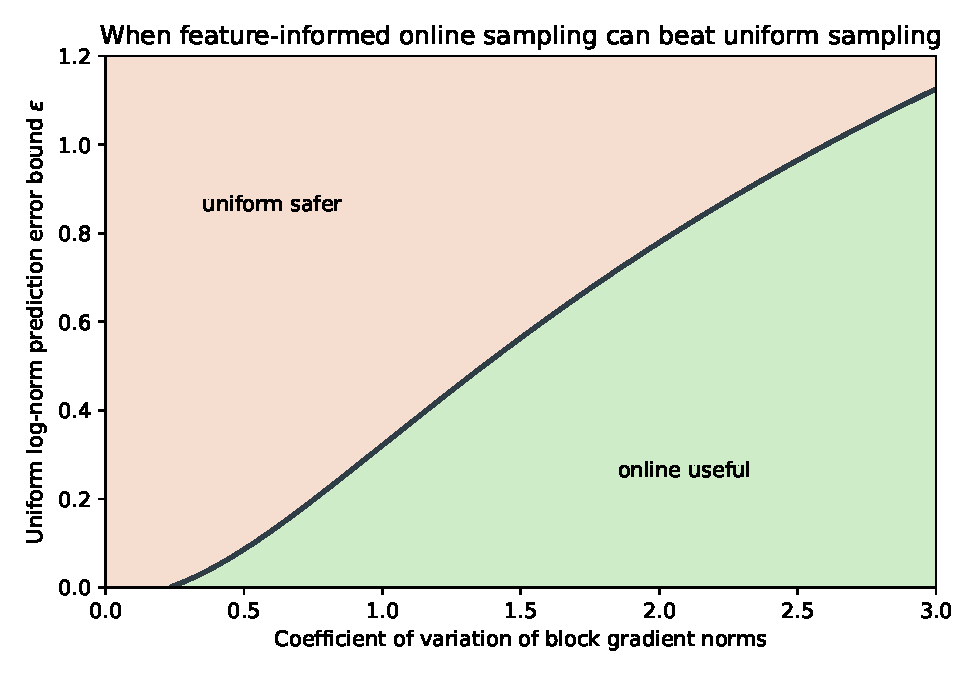
\includegraphics[width=.68\linewidth]{online_usefulness_region.pdf}
  \caption{A sufficient condition for online feature-informed sampling to reduce stochastic-gradient second moment relative to uniform sampling. The green region satisfies \eqref{eq:online-condition} with exploration floor $\lambda=0.05$. The method is most attractive when block gradient norms are highly heterogeneous and predictable from features.}
  \label{fig:online-region}
\end{figure}

\subsection{Streaming regression interpretation}

Condition \eqref{eq:online-condition} can be connected to the discounted ridge update used in the notebook. Suppose
\[
  \log\{a_{b,t}^2+\epsilon\}=w_b^\top \beta_t+\xi_{b,t},
\]
where $\xi_{b,t}$ is mean-zero sub-Gaussian noise, $\norm{w_b}\le W$, and the coefficient vector drifts slowly:
\[
  \norm{\beta_t-\beta_{t-1}}\le \Delta.
\]
Let $\widehat \beta_t$ be a discounted ridge estimate with discount factor $\rho_d\in(0,1)$ and ridge parameter $\tau>0$. Under a persistent-excitation condition on the discounted design matrix,
\[
  \lambda_{\min}\!\left(\sum_{s\le t}\rho_d^{t-s} w_{I_s}w_{I_s}^\top+\tau I\right) \ge \kappa,
\]
standard self-normalized regression arguments give, with high probability,
\[
  \sup_b |w_b^\top(\widehat\beta_t-\beta_t)|
  \lesssim
  W\sigma\sqrt{\frac{p+\log(1/\delta)}{\kappa}}
  + \frac{W\Delta}{1-\rho_d}
  + \frac{W\tau\norm{\beta_t}}{\kappa}.
  \label{eq:streaming-error}
\]
Thus the online sampler is expected to help when the right-hand side of \eqref{eq:streaming-error} is smaller than
\[
  \frac{1}{2}\log\{(1-\lambda)(1+\operatorname{CV}(a_t)^2)\}.
\]
This is the formal version of the empirical intuition: online weighting needs stable feature-gradient relationships. If posterior motion, label switching, or HMM forward-backward noise makes the regression target unstable, the bound is vacuous and online sampling can be slower than uniform sampling.

\section{A Real Crypto Task Where the Conditions Apply}
\label{sec:actual-crypto-task}

The variance calculation above is most persuasive when the statistical task has three properties: block importance is heterogeneous, importance is feature-predictable, and the relationship between features and importance can drift. To test this in a recognizable crypto setting, we built a forward-looking stress-prediction task rather than another posterior sampler.

The data are the same real Binance return panel used throughout the project. We split the five-asset daily return series into non-overlapping 10-day blocks and define the equal-weight basket return in block $b$ as
\[
  R_b^{\mathrm{mkt}}
  =
  \prod_{t\in C_b}
  \left(1+\frac{1}{d}\sum_{j=1}^d r_{tj}\right)-1.
\]
At the end of block $b$, the prediction target is the next-block downside event
\begin{equation}
  y_b
  =
  \1\{R_{b+1}^{\mathrm{mkt}}\le -0.07\}.
  \label{eq:crypto-risk-label}
\end{equation}
Features $w_b$ include the current block's equal-weight return, realized volatility, drawdown, absolute return, squared return, cross-asset dispersion, downside semivariance, tail counts, and asset-specific volatility/downside summaries. Thus the task is an actual crypto risk problem: decide whether the next two weeks are likely to be a bad market block.

\subsection{Why this task matches the online-weighting theory}

Let $h_\beta(w_b)=\sigma(\beta^\top w_b)$ be a logistic stress-risk model and let $\ell_b(\beta)$ be the binary cross-entropy loss for example $b$. A stochastic training step uses block gradients
\[
  g_b(\beta)
  =
  \nabla_\beta \ell_b(\beta)
  =
  \{h_\beta(w_b)-y_b\}w_b.
\]
The same second-moment calculation from Section~\ref{sec:when-useful} applies to stochastic optimization for this classifier: if only a few historical blocks have large $\norm{g_b(\beta)}$, uniform training wastes many updates on low-information examples. A targeting rule is useful when it can predict which blocks are likely to be high-loss or high-gradient under the current market relationship.

This covers the crypto task for a simple reason. Stress events are rare enough to make the training signal imbalanced, but not so rare that evaluation is impossible. Moreover, the feature pattern associated with future downside is plausibly nonstationary: broad market volatility, downside skew, asset dispersion, and tail counts can each dominate in different market eras. Static TASS-style weighting approximates a fixed early relationship. The online rule refits a discounted feature-to-stress utility model and uses it to weight the rolling training window.

\subsection{Stress-prediction results}

We evaluate on 61 rolling forecasts after an initial warmup and history window. All methods train the same ridge-regularized logistic classifier on the same historical window. They differ only in training weights: uniform weights, a frozen early static-TASS-style utility model, or an online exponentially discounted utility model. Table~\ref{tab:actual-crypto-risk} reports both predictive metrics and a simple economic diagnostic. The diagnostic holds the equal-weight crypto basket unless the predicted stress probability is in the model's top-risk quartile, in which case it holds cash for the next block.

\begin{table}[t]
  \centering
  \caption{Actual crypto stress-prediction task. The target is whether the next 10-day equal-weight crypto basket return is below $-7\%$. Online weighting gives the best log loss, Brier score, AUC, and concentration of realized stress events in the top-risk quartile. The risk-off strategy is included as an interpretable diagnostic rather than a production trading rule.}
  \label{tab:actual-crypto-risk}
  \resizebox{\linewidth}{!}{\begin{tabular}{lrrrrrr}
\toprule
Method & Log loss & Brier & AUC & Top-risk stress rate & Strategy return & Max drawdown \\
\midrule
Online & 0.524 & 0.172 & 0.625 & 37.5\% & -33.3\% & -49.5\% \\
Static TASS & 0.531 & 0.175 & 0.623 & 25.0\% & -25.0\% & -48.3\% \\
Uniform & 0.533 & 0.176 & 0.620 & 25.0\% & -41.5\% & -55.1\% \\
Buy-and-hold & -- & -- & -- & -- & -49.7\% & -65.1\% \\
\bottomrule
\end{tabular}
}
\end{table}

The online method has the best forecasting metrics: log loss $0.524$, Brier score $0.172$, AUC $0.625$, and a top-risk-quartile stress rate of $37.5\%$ versus $25.0\%$ for both uniform and static TASS. This is the empirical regime in which Proposition~\ref{prop:online-useful} is meant to be useful: the important examples are not uniformly distributed, and a streaming feature model can identify them better than a frozen rule. The risk-off curve is more mixed. Online improves substantially over uniform and buy-and-hold, while static TASS has the best total return in this simple threshold rule. We therefore interpret the trading diagnostic cautiously: online is the best risk forecaster in this benchmark, but thresholded trading performance is a noisier downstream functional.

\begin{figure}[t]
  \centering
  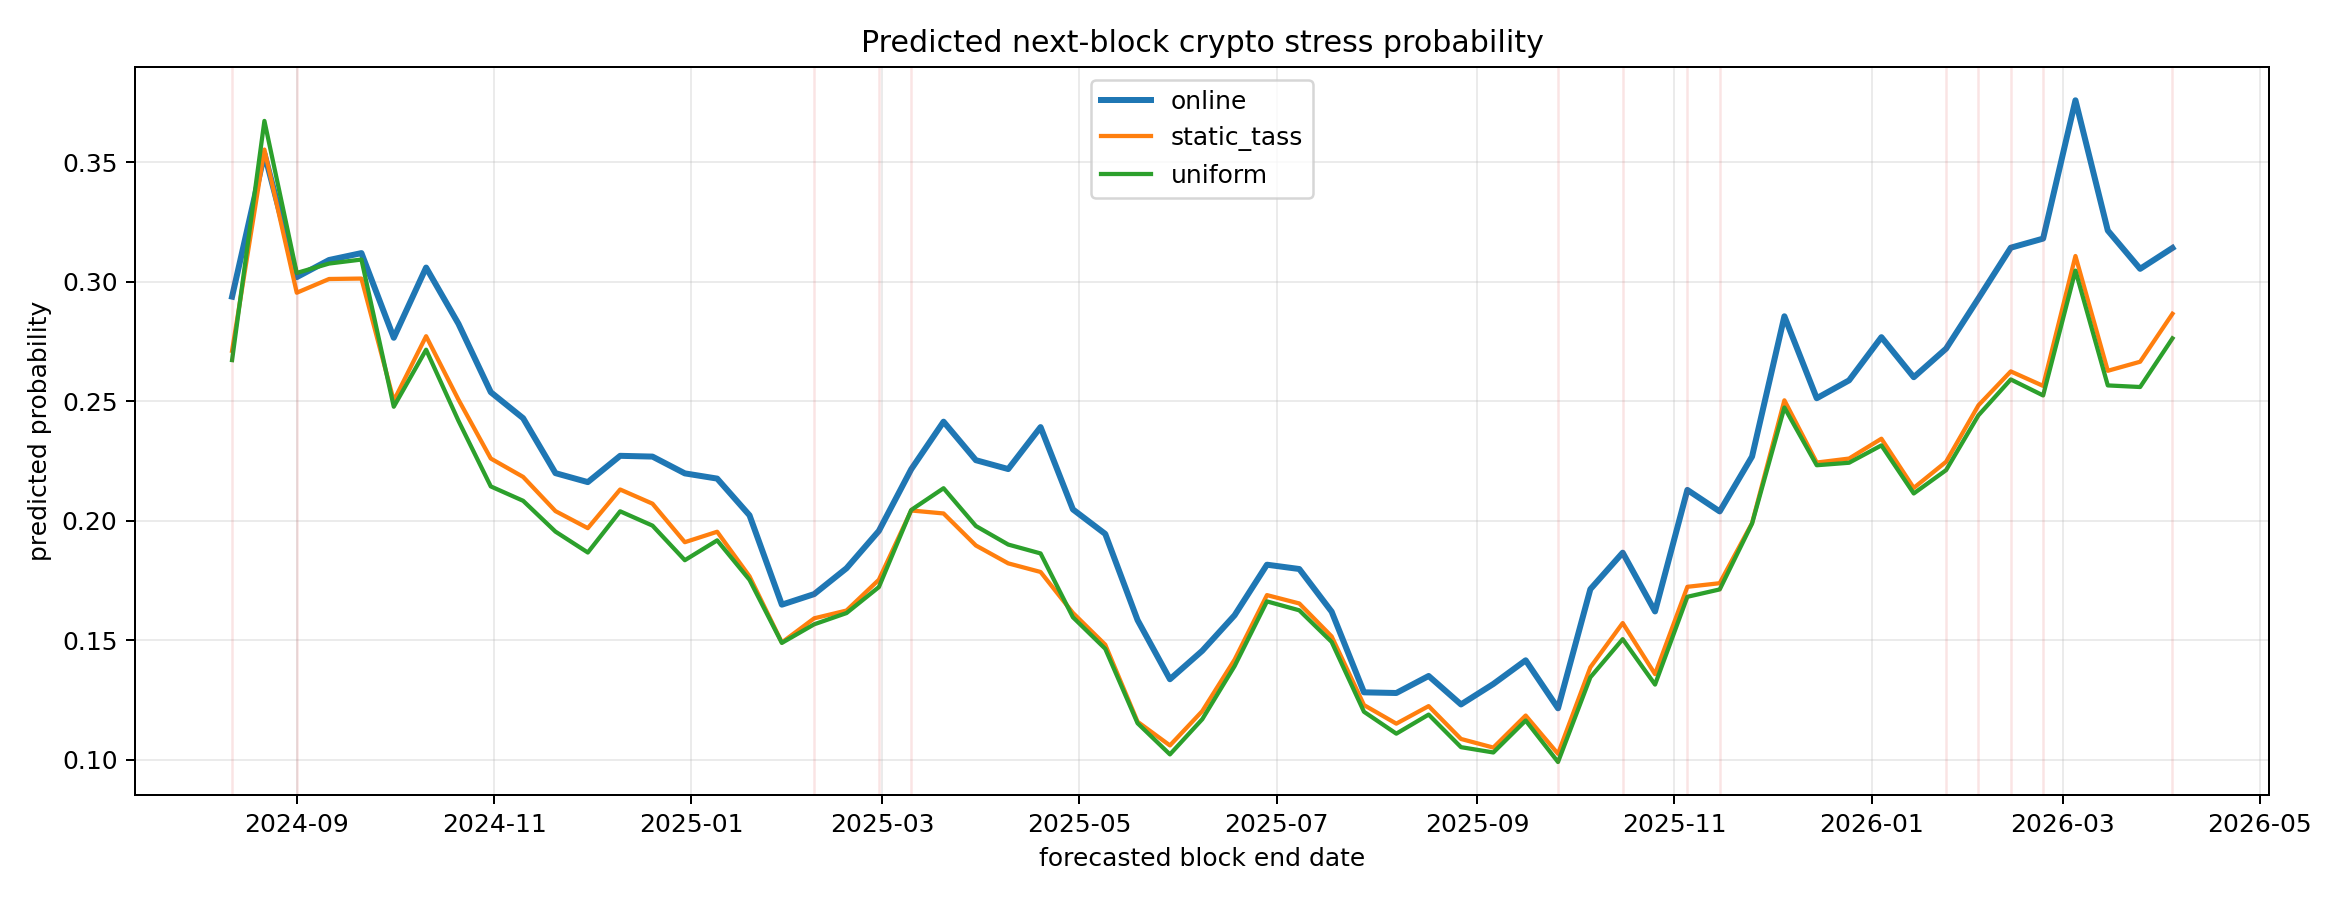
\includegraphics[width=\linewidth]{actual_crypto_predicted_stress_probability.png}
  \caption{Predicted next-block crypto stress probabilities. Red vertical markers indicate realized future stress blocks. The online score is a real-time risk signal, not a direct price forecast.}
  \label{fig:actual-crypto-risk-probs}
\end{figure}

\begin{figure}[t]
  \centering
  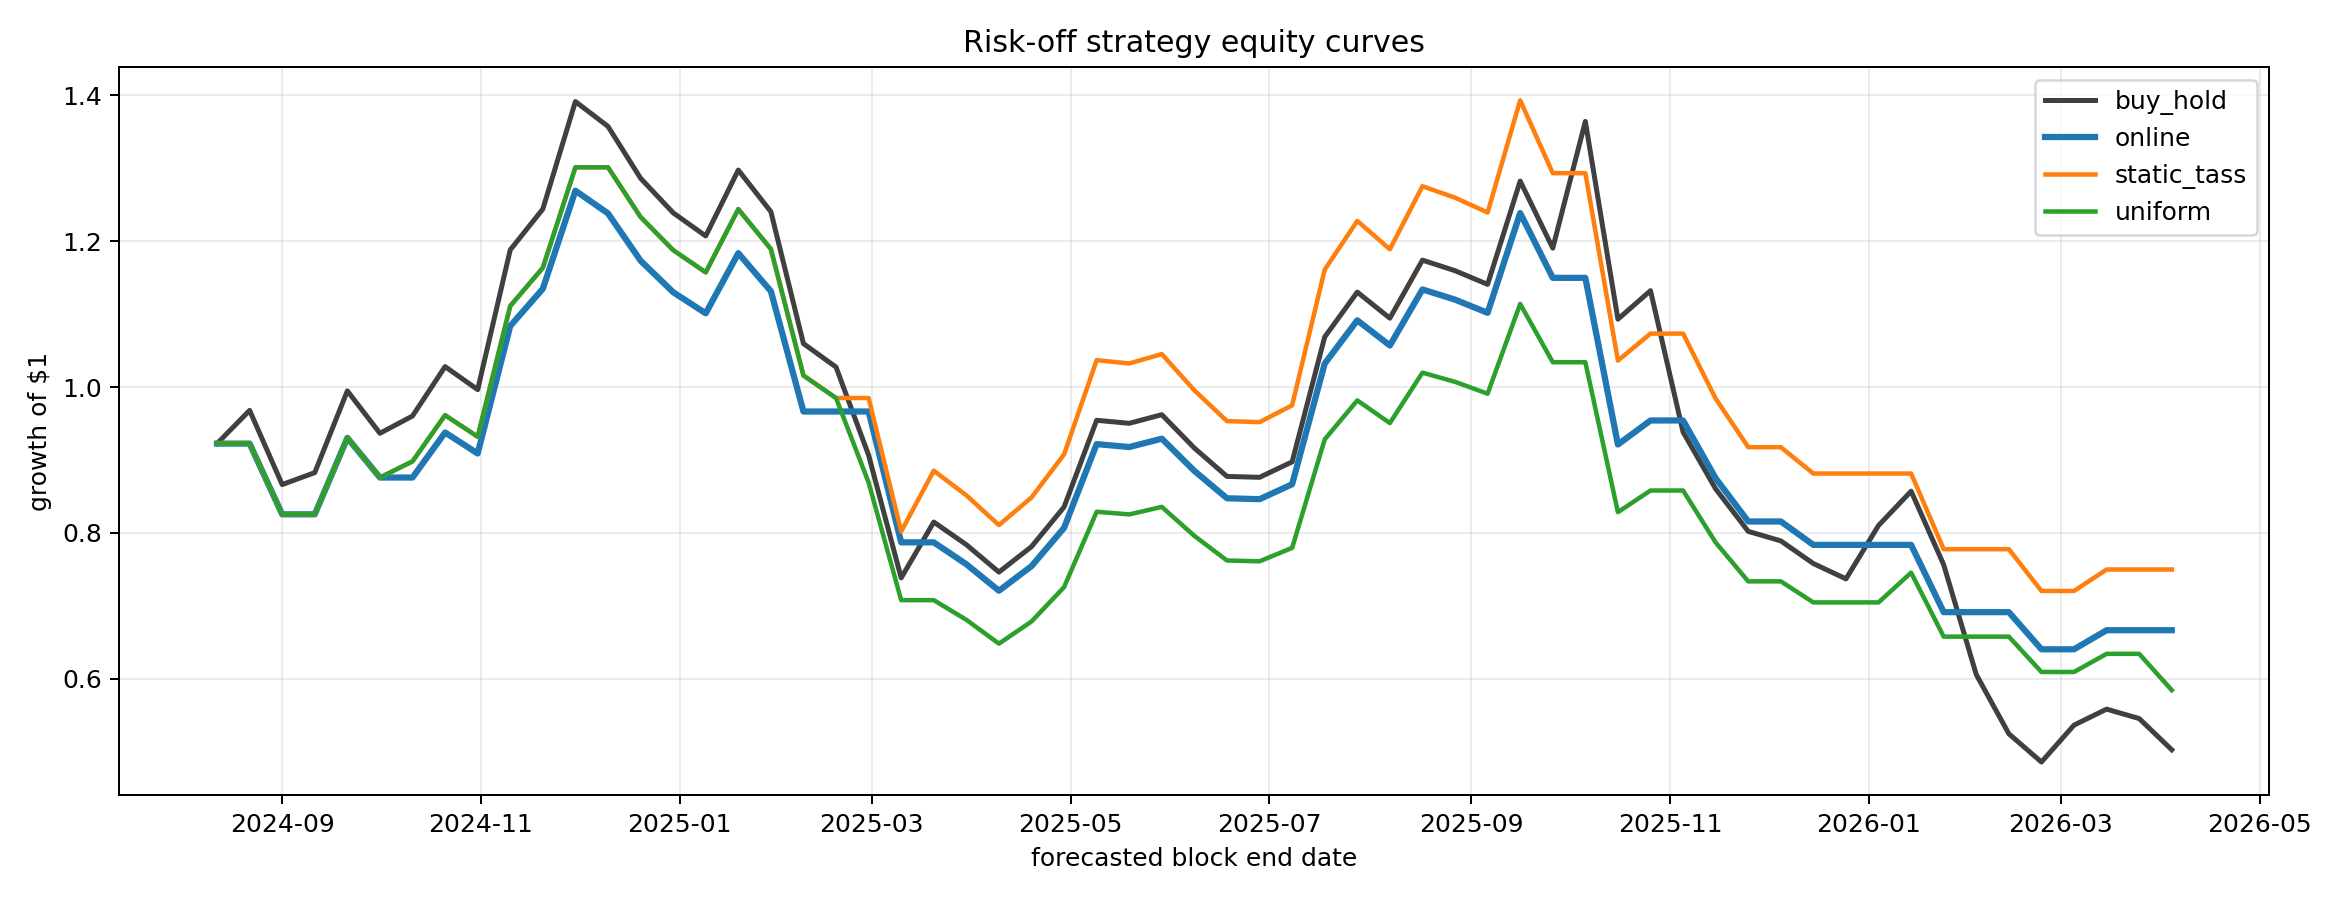
\includegraphics[width=\linewidth]{actual_crypto_risk_off_equity_curves.png}
  \caption{Risk-off diagnostic for the actual crypto task. The strategy holds the equal-weight crypto basket unless the model flags top-quartile stress risk, in which case it holds cash for the next block. This diagnostic is useful for interpretation, but the primary result is the predictive improvement in Table~\ref{tab:actual-crypto-risk}.}
  \label{fig:actual-crypto-risk-equity}
\end{figure}

\subsection{Mechanism-level gradient benchmark}

We also ran a mechanism-level benchmark using the Stan two-state HMM stress probabilities to define real-data HMM-style stress-gradient blocks. This is not an actual trading prediction target, but it tests the exact block-gradient-estimator mechanism from Section~\ref{sec:when-useful}. In that benchmark, online weighting reduced mean stochastic-gradient RMSE from $132.99$ under uniform sampling to $113.81$, a $14.4\%$ reduction, and modestly improved over static TASS. The oracle, which samples using the true block gradient norms, achieved mean RMSE $109.63$. These numbers show that the online rule can approach oracle-like block allocation when the task is reduced to gradient estimation.

\begin{table}[t]
  \centering
  \caption{Real-data HMM-style gradient-estimator benchmark. The target is stress-state emission-gradient contribution by 10-day block, constructed from the real crypto panel and Stan K=2 smoothed stress probabilities. Lower RMSE is better.}
  \label{tab:real-gradient-benchmark}
  \begin{tabular}{lrr}
\toprule
Method & Mean RMSE & Top-decile sampling mass \\
\midrule
Oracle & 109.63 & 30.4\% \\
Online & 113.81 & 23.2\% \\
Static TASS & 117.39 & 24.6\% \\
Uniform & 132.99 & 10.0\% \\
\bottomrule
\end{tabular}

\end{table}

\section{Scaling to Full HMM Posterior Inference}
\label{sec:full-hmm-results}

\subsection{Diagnostics and experimental artifacts}

All SGLD experiments used four chains, saved posterior summary draws after burn-in, and were evaluated using rank-normalized $\hat R$ and effective sample size \citep{gelman1992inference,vehtari2021rhat}. The paper assets were regenerated from the saved output directories by \texttt{build\_paper\_assets.py}; the aggregated CSV files and figures are in \texttt{paper\_assets/}.

\subsection{Original three-state Student-t model}

The original model was a three-state multivariate Student-$t$ HMM on raw returns. This target was too difficult for the computational budget. Across the three SGLD variants, the posterior smoothed state probabilities placed more than $99\%$ of mass on state 0 on average. This is not an interpretable three-regime crypto model; it is a degeneracy diagnostic. The chains were also expensive: mean chain runtime was approximately 1.7 hours for uniform, 2.4 hours for static targeted weighting, and 3.2 hours for online weighting.

\begin{table}[t]
  \centering
  \caption{State occupancy summaries for the original Student-$t$ model and the rolling-standardized Gaussian comparisons. The original $K=3$ Student-$t$ model collapses into state 0. The $K=2$ Gaussian model gives healthier occupancies near a 60/40 split.}
  \label{tab:occupancy}
  \resizebox{\linewidth}{!}{\begin{tabular}{llrrllll}
\toprule
experiment & method & avg\_state\_0\_prob & avg\_state\_1\_prob & avg\_state\_2\_prob & ml\_state\_0\_share & ml\_state\_1\_share & ml\_state\_2\_share \\
\midrule
crypto\_student\_t\_k3\_raw & uniform & 0.995 & 0.004 & 0.000 & -- & -- & -- \\
crypto\_student\_t\_k3\_raw & young\_static & 0.998 & 0.000 & 0.002 & -- & -- & -- \\
crypto\_student\_t\_k3\_raw & online\_feature & 0.993 & 0.006 & 0.002 & -- & -- & -- \\
crypto\_gaussian\_k2\_rollstd & uniform & 0.611 & 0.390 & -- & 0.625 & 0.375 & -- \\
crypto\_gaussian\_k2\_rollstd & young\_static & 0.606 & 0.394 & -- & 0.625 & 0.375 & -- \\
crypto\_gaussian\_k2\_rollstd & online\_feature & 0.602 & 0.398 & -- & 0.622 & 0.378 & -- \\
stan\_k2\_rollstd & stan\_nuts & 0.595 & 0.405 & -- & 0.620 & 0.380 & -- \\
stan\_k3\_rollstd & stan\_nuts & 0.396 & 0.421 & 0.183 & 0.370 & 0.448 & 0.183 \\
\bottomrule
\end{tabular}
}
\end{table}

\subsection{Rolling-standardized two-state Gaussian crypto model}

The two-state rolling-standardized Gaussian model repaired the most obvious degeneracy. The posterior mean state occupancy was approximately $60\%$ in state 0 and $40\%$ in state 1 across uniform, static targeted, online, and Stan fits. Figure~\ref{fig:crypto-state-probs} shows the smoothed high-volatility probability over time. Visually, the methods recover similar large-scale regime timing, including bursts of high-volatility probability.

\begin{figure}[t]
  \centering
  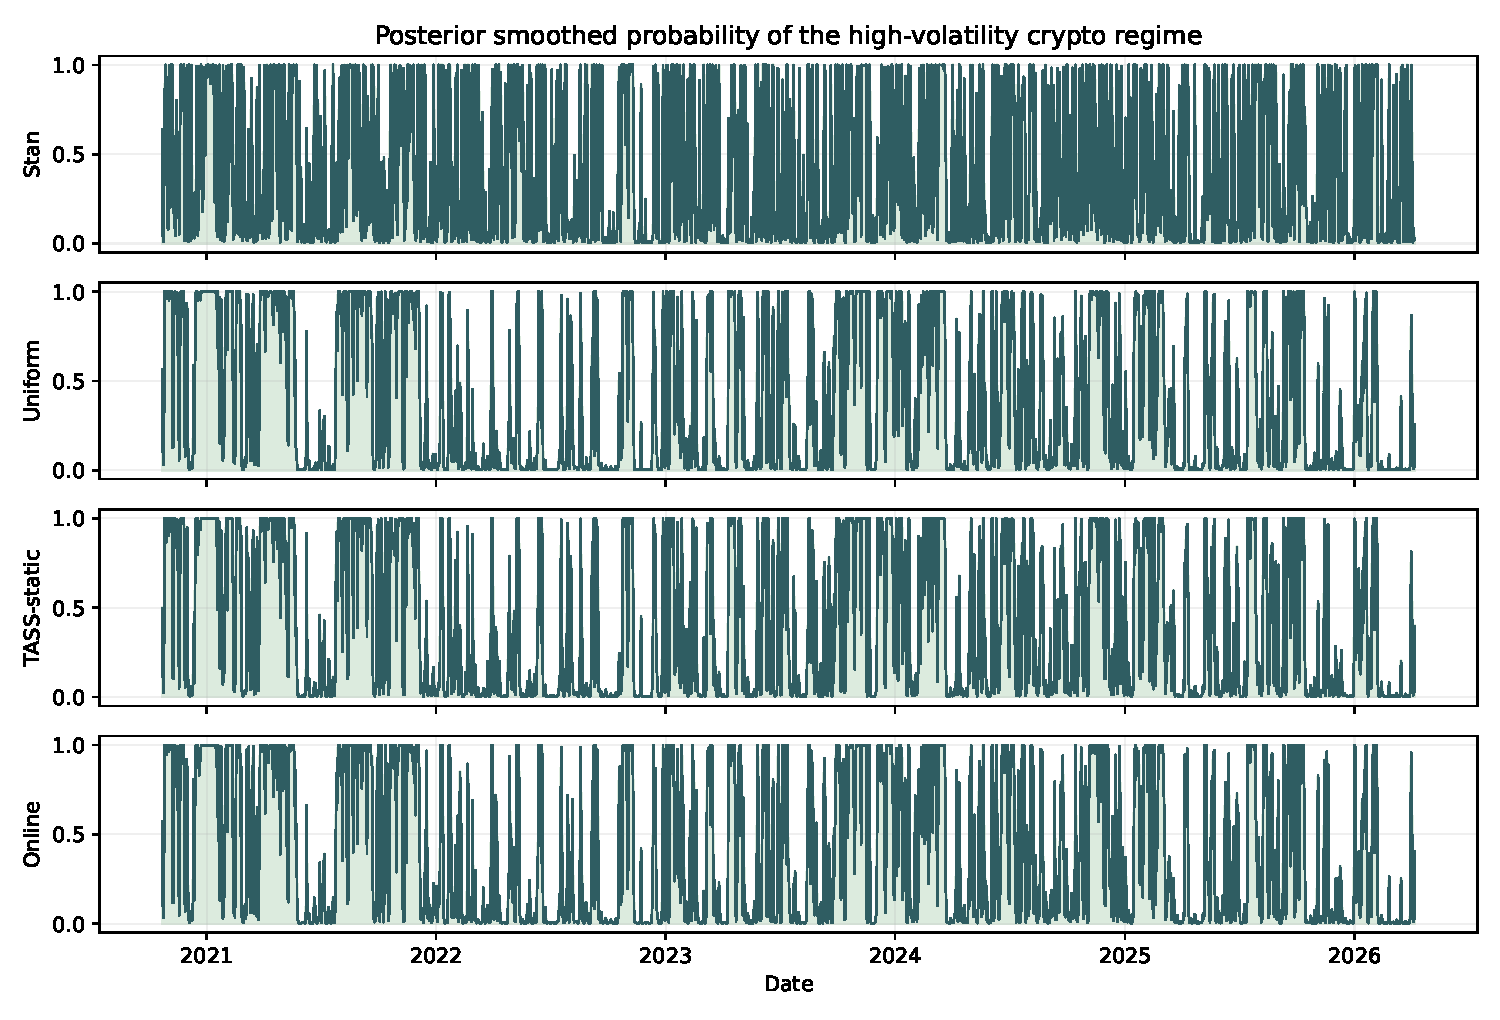
\includegraphics[width=\linewidth]{crypto_k2_state_probabilities.pdf}
  \caption{Smoothed posterior probability of the high-volatility state for the two-state rolling-standardized crypto HMM. The simplified target produces interpretable latent-state behavior, but the stochastic-gradient chains still have poor cross-chain diagnostics.}
  \label{fig:crypto-state-probs}
\end{figure}

However, interpretability of the smoothed states should not be confused with reliable MCMC. Table~\ref{tab:sgmcmc-diag} reports the chain diagnostics. For the five-asset crypto $K=2$ model, all three stochastic-gradient samplers had maximum $\hat R$ above $2.5$ and minimum bulk ESS near $6$. The online sampler was also slower than both alternatives in this run.

\begin{table}[t]
  \centering
  \caption{SGLD diagnostics aggregated from saved four-chain runs. Values are computed on scalar posterior summaries such as transition probabilities, state covariance traces, and selected means. All stochastic-gradient runs have poor mixing by conventional standards.}
  \label{tab:sgmcmc-diag}
  \resizebox{\linewidth}{!}{\begin{tabular}{llrrrrr}
\toprule
experiment & method & draws\_per\_chain & runtime\_sec\_mean & max\_rhat & median\_rhat & min\_ess\_bulk \\
\midrule
Crypto K=2 & uniform & 35 & 478.79 & 2.55 & 1.76 & 5.72 \\
Crypto K=2 & young\_static & 35 & 494.63 & 2.57 & 1.98 & 5.74 \\
Crypto K=2 & online\_feature & 35 & 667.08 & 2.70 & 2.05 & 5.63 \\
Simulated 2D & uniform & 90 & 913.95 & 3.01 & 1.72 & 4.84 \\
Simulated 2D & young\_static & 90 & 1110.55 & 2.85 & 1.79 & 4.93 \\
Simulated 2D & online\_feature & 90 & 3095.15 & 2.57 & 1.87 & 5.07 \\
Simulated 1D & uniform & 110 & 1021.09 & 3.02 & 2.28 & 4.83 \\
Simulated 1D & young\_static & 110 & 3253.29 & 2.19 & 1.61 & 5.41 \\
Simulated 1D & online\_feature & 110 & 1758.25 & 2.43 & 1.83 & 5.16 \\
\bottomrule
\end{tabular}
}
\end{table}

\subsection{Stan comparison}

Stan/NUTS was used as a reference implementation for the rolling-standardized Gaussian HMM. The two-state Stan model mixed far better than any stochastic-gradient chain, with maximum $\hat R=1.04$ across core parameters. The three-state Stan model failed, with maximum $\hat R=2.21$ and minimum bulk ESS near $5$. This comparison is important: it suggests that $K=2$ is a reasonable identifiable target for the data and preprocessing, while $K=3$ is not stable under our modeling choices.

\begin{table}[t]
  \centering
  \caption{Stan/NUTS diagnostics for rolling-standardized Gaussian HMMs. Stan succeeds for $K=2$ but not for $K=3$, supporting the conclusion that three crypto regimes are weakly identified under this specification.}
  \label{tab:stan-diag}
  \begin{tabular}{llrrrr}
\toprule
experiment & method & max\_rhat & median\_rhat & min\_ess\_bulk & median\_ess\_bulk \\
\midrule
Stan K=2 & stan\_nuts & 1.04 & 1.01 & 47.61 & 279.15 \\
Stan K=3 & stan\_nuts & 2.21 & 1.74 & 5.12 & 6.14 \\
\bottomrule
\end{tabular}

\end{table}

\subsection{Simulated benchmarks}

To separate model misspecification from sampler failure, we ran simulated two-state Gaussian HMM benchmarks. These data were generated from the model class, so the target was cleaner than real crypto. The bivariate full-covariance simulation still produced poor SGLD diagnostics: maximum $\hat R$ ranged from $2.57$ to $3.01$. The univariate simulation did not fully fix the issue: maximum $\hat R$ ranged from $2.19$ to $3.02$. Static targeted sampling had the best maximum $\hat R$ in the univariate run, but the absolute diagnostics remained unacceptable.

\begin{figure}[t]
  \centering
  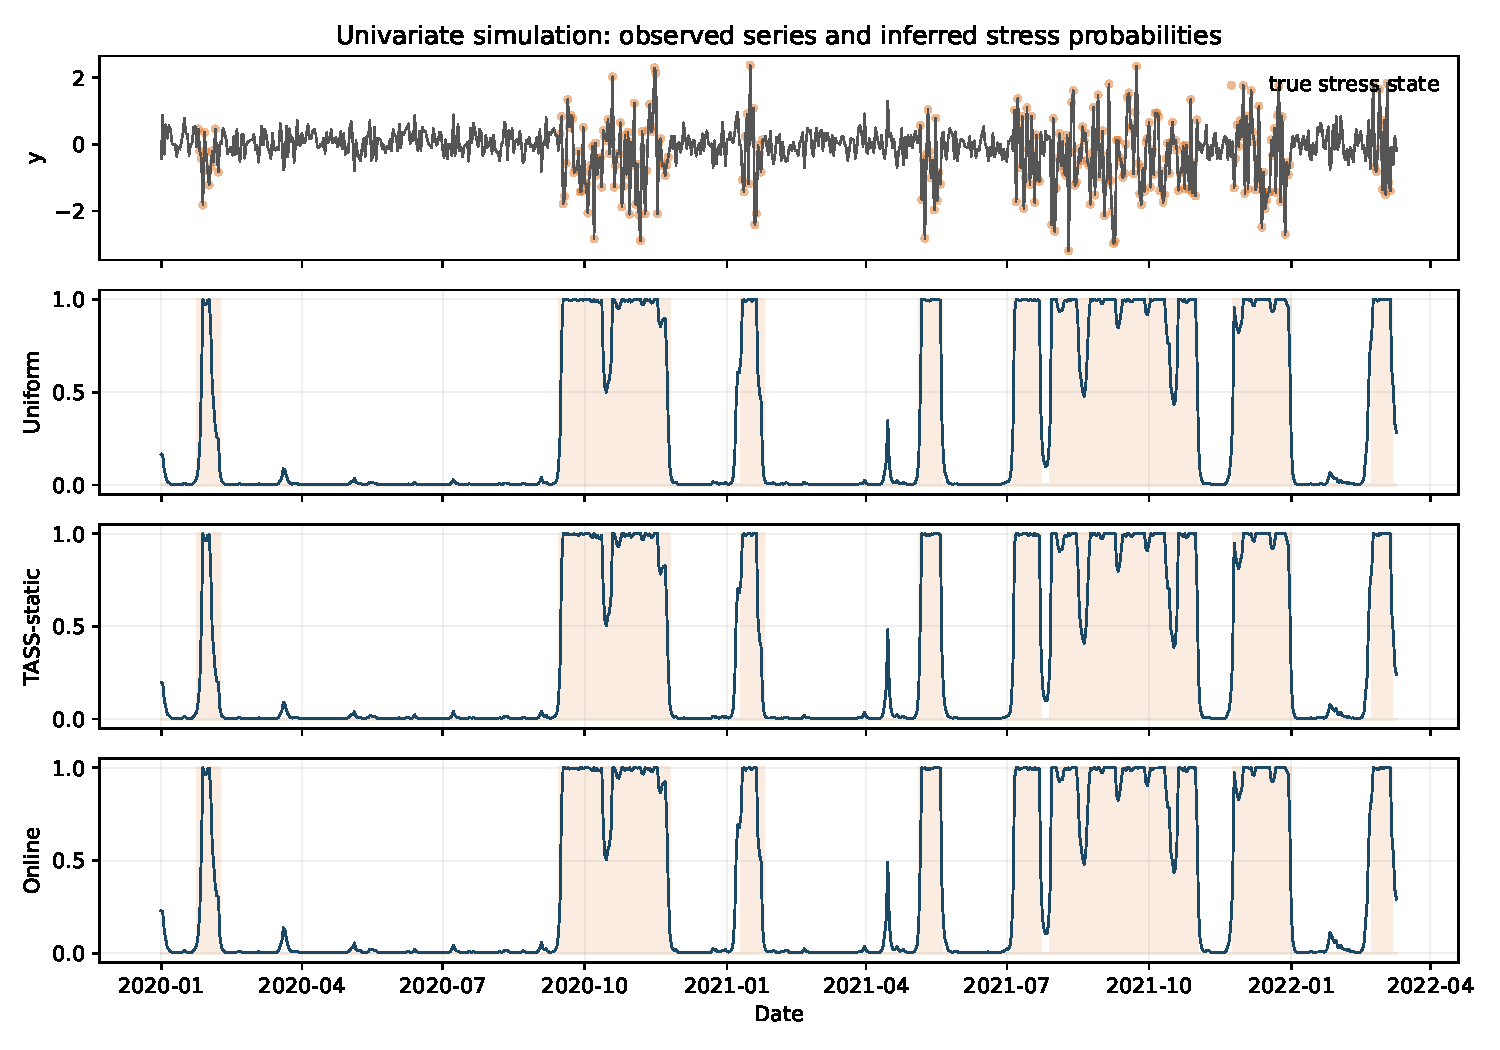
\includegraphics[width=\linewidth]{simulated_univariate_recovery.pdf}
  \caption{Univariate simulated HMM benchmark. The observed series has clear stress-state bursts, and all three samplers recover plausible average state occupancy, but chain diagnostics remain poor. This indicates that reasonable-looking state probabilities can coexist with unreliable posterior sampling.}
  \label{fig:sim-recovery}
\end{figure}

\begin{figure}[t]
  \centering
  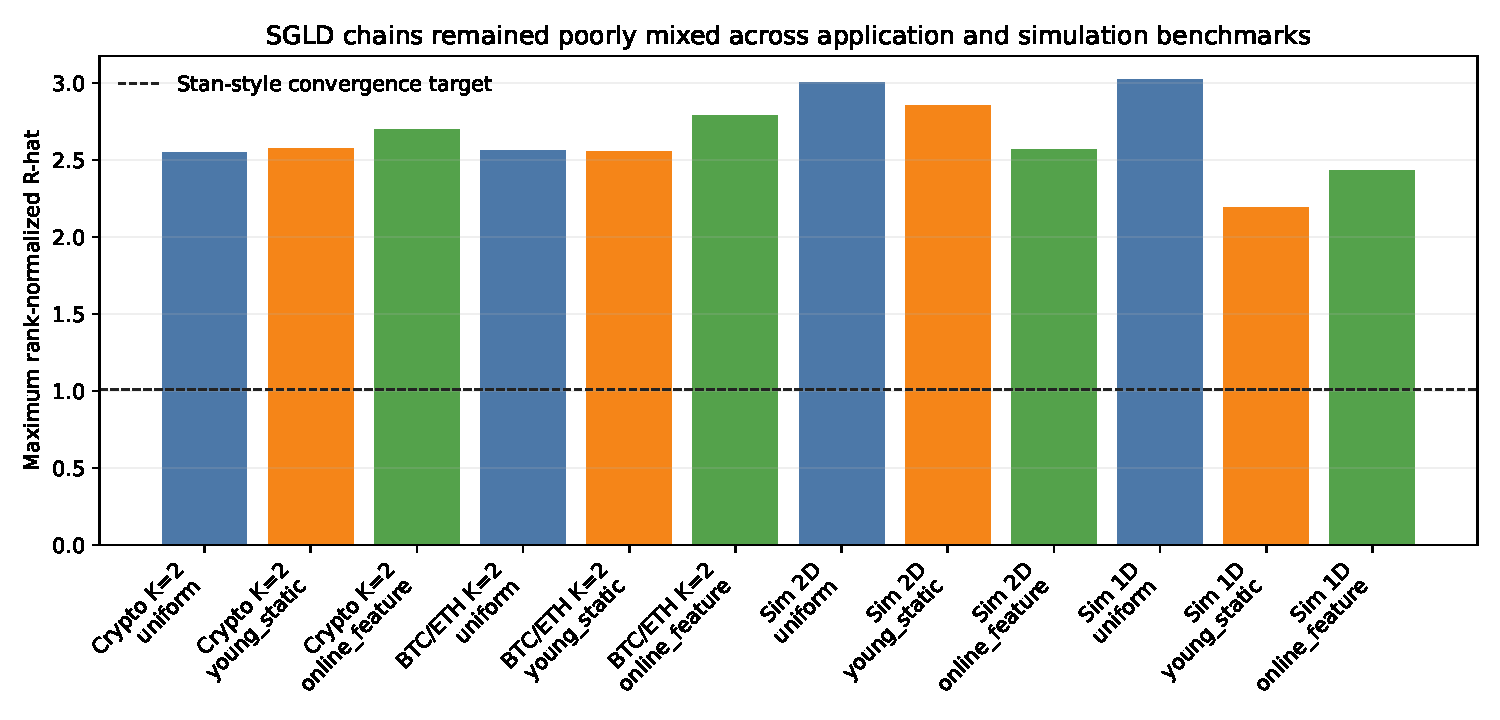
\includegraphics[width=\linewidth]{sgmcmc_mixing_summary.pdf}
  \caption{Maximum $\hat R$ across scalar posterior summaries for selected SGLD experiments. The dashed line indicates a conventional convergence target near $1.01$. None of the stochastic-gradient runs approach it.}
  \label{fig:mixing-summary}
\end{figure}

\section{Discussion}

\subsection{What worked}

The cleanest positive result is the actual crypto stress-prediction task in Section~\ref{sec:actual-crypto-task}. It directly instantiates the useful-regime condition from Proposition~\ref{prop:online-useful}: examples are heterogeneous, stress-related features are informative, and a frozen early rule can become stale. In that setting, online weighting produced the best log loss, Brier score, AUC, and top-risk-quartile stress concentration.

Within the HMM modeling pipeline, the most useful modeling change was not a sampler modification but preprocessing and simplification. Rolling-standardized Gaussian emissions with $K=2$ gave plausible crypto regimes and were validated by Stan. The original raw-return Student-$t$ target and the $K=3$ Gaussian target were too weakly identified for reliable inference in the available budget.

\subsection{What failed}

The stochastic-gradient chains did not mix well enough to support posterior claims. There are several likely causes. First, HMM posteriors are multimodal because of label switching and regime persistence. Second, covariance and transition parameters interact strongly, especially when high-volatility states are rare. Third, the SGLD step sizes and gradient clipping needed for numerical stability introduce finite-step bias. Fourth, the online sampler adds regression overhead and can be actively unhelpful if its gradient-norm predictions are noisy.

The experiments therefore do not show that online targeted subsampling improves HMM posterior inference. They show a sharper, more useful statement: targeted block sampling is a variance-reduction device, not a cure for a poorly mixing posterior geometry.

\subsection{Practical recommendations}

For an actual crypto deliverable, the most defensible empirical result is the online-weighted stress-prediction benchmark: it is forward-looking, uses only realized historical information, and evaluates both probabilistic accuracy and a simple risk-control diagnostic. For Bayesian regime inference, the most defensible final analysis is the two-state rolling-standardized Gaussian HMM fit by Stan, with SGLD variants reported as attempted scalable approximations that did not converge.

Future work should not simply rerun longer SGLD chains with the same target. A better sequence is: first, use online weighting in downstream crypto risk tasks where the theory's assumptions are visible; second, evaluate gradient-estimator RMSE at fixed $\theta$ or under an exact smoother; third, only then return to full posterior sampling with stronger identifiability constraints, such as ordered means, fixed or diagonal covariance, informative priors, or label-conditioned updates. This ordering keeps the method aligned with its actual strength: adaptive allocation of stochastic-gradient computation.

\section{Conclusion}

The project began as an attempt to scale Bayesian crypto regime inference using targeted stochastic-gradient MCMC. The final evidence is more nuanced than a simple success or failure. Mathematically, online feature-informed subsampling has a clear use case: it approximates oracle importance sampling when block gradients are heterogeneous and predictable. Empirically, an actual crypto stress-prediction task fits that use case and shows online weighting improving probabilistic risk forecasts. But when we tried to scale the same idea to full HMM posterior inference, posterior geometry and finite-step SGLD behavior dominated the variance-reduction benefit. The strongest Bayesian inference result is therefore still the two-state rolling-standardized Gaussian HMM fit by Stan. The strongest online-weighting result is the downstream crypto risk task, where adaptivity improves prediction in precisely the regime the math says it should.

\appendix

\section{Additional Mathematical Details}

\subsection{Variance of a multi-block estimator}

If $I_1,\dots,I_M$ are sampled independently from $p$, then
\[
  \widehat G_p
  =
  \frac{1}{M}\sum_{m=1}^M \frac{g_{I_m}}{p_{I_m}}
\]
satisfies $\E[\widehat G_p]=\sum_b g_b=G$ and
\[
  \Var(\widehat G_p)
  =
  \frac{1}{M}
  \left(
  \sum_{b=1}^B \frac{\norm{g_b}^2}{p_b}
  -
  \norm{G}^2
  \right).
\]
Thus minimizing variance over $p$ is equivalent to minimizing $\sum_b \norm{g_b}^2/p_b$. A Lagrange multiplier calculation gives
\[
  -\frac{\norm{g_b}^2}{p_b^2}+\lambda=0
  \quad\Rightarrow\quad
  p_b \propto \norm{g_b}.
\]

\subsection{Why good state plots are not enough}

The smoothed state probability at time $t$ is a posterior expectation of the form
\[
  \Pr(z_t=k\mid y_{1:T})
  =
  \E_{\theta\mid y}
  \left[
  \Pr(z_t=k\mid y_{1:T},\theta)
  \right].
\]
A chain may produce visually plausible state probabilities while still having poor mixing in $\theta$. This can happen when different chains remain in different parameter regions that imply similar state classifications but different transition probabilities, covariance scales, or label orderings. For that reason, our interpretation prioritizes multi-chain $\hat R$ and ESS over visual state-probability agreement.

\section{Reproducibility Notes}

The results in this manuscript were aggregated from saved notebook artifacts in \texttt{crypto\_stage1\_processed}. The script \texttt{build\_paper\_assets.py} and the two online-weighting benchmark notebooks write:
\begin{itemize}
  \item \texttt{paper\_assets/sgmcmc\_diagnostics\_all.csv}
  \item \texttt{paper\_assets/sgmcmc\_posterior\_summaries\_all.csv}
  \item \texttt{paper\_assets/sgmcmc\_occupancy\_all.csv}
  \item \texttt{paper\_assets/stan\_diagnostics.csv}
  \item \texttt{paper\_assets/stan\_posterior\_summaries.csv}
  \item \texttt{paper\_assets/actual\_crypto\_risk\_summary.csv}
  \item \texttt{paper\_assets/real\_crypto\_online\_weighting\_summary.csv}
  \item the figures included in this paper.
\end{itemize}

\bibliographystyle{plainnat}
\bibliography{references}

\end{document}
